In this lab we will be performing a Man-in-the-Middle (MitM) attack using the 3 virtual machines listed below:
\begin{table}[H]
    \centering\begin{tabular}{c l l l}
        \textbf{Sr} & \textbf{System} & \textbf{IP Address} & \textbf{Physical Address} \\
        \hline
        1 & Windows-10 & 192.168.56.104 & 08-00-27-56-34-4E\\
        2 & Windows-10 Clone & 192.168.56.103 & 08-00-27-0E-13-8A\\
        3 & Kali-Linux & 192.168.56.102 & 08-00-27-44-48-d7
    \end{tabular}
    \caption{Address list for the VMs.}
    \label{tab:address-list}
\end{table}

First we establish a connection between the two Windows machines using the ping command.
Pings were not being returned between the Windows machines so I had to disable the Windows Defender Firewall to allow the traffic.

\begin{figure}[H]
    \centering
    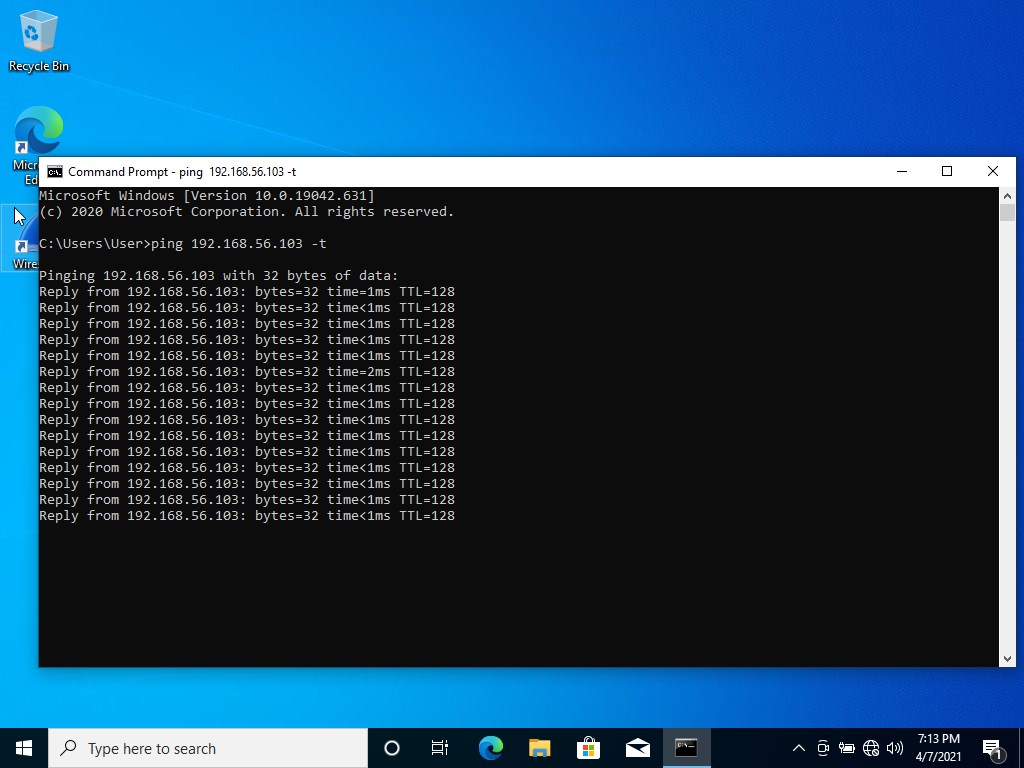
\includegraphics[width=\linewidth]{figures/ping-initial.png}
    \caption{Starting the connection between the Windows-10 and Windows-10 Clone machines.}
    \label{fig:ping-initial}
\end{figure}

In the Kali machine we open up Wireshark to monitor the network traffic.
The promiscuous mode needs to be set on the VirtualBox host-only network adapter to see other VM traffic.

\begin{figure}[H]
    \centering
    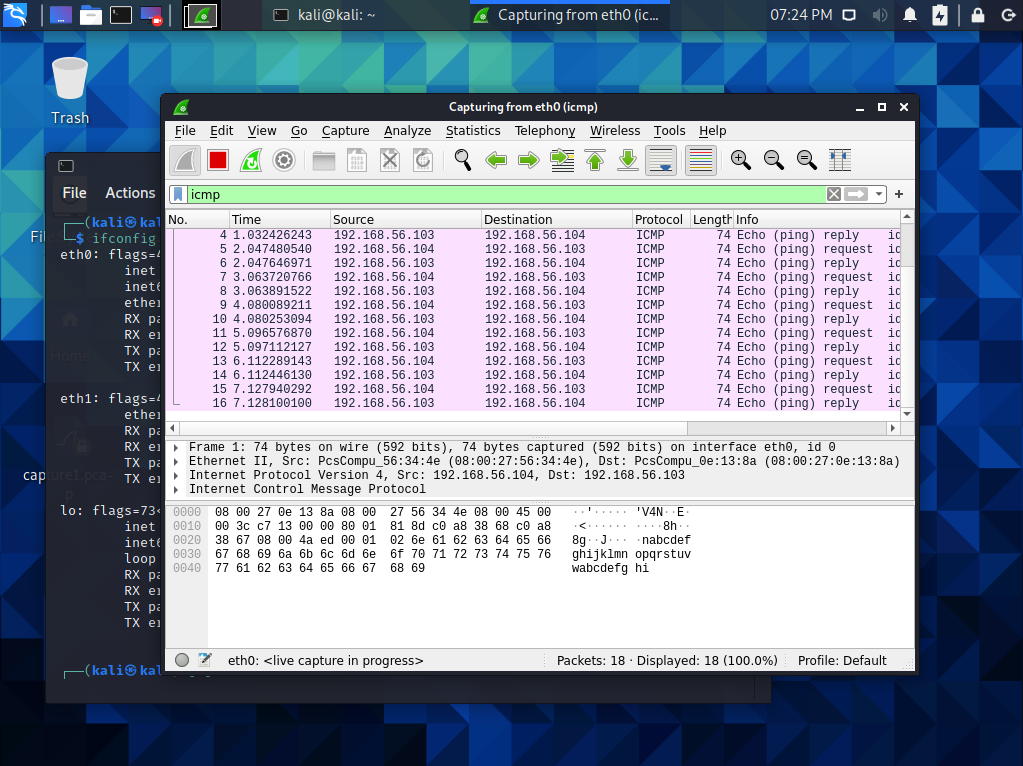
\includegraphics[width=\linewidth]{figures/wireshark-initial.png}
    \caption{Capturing the packets between the two Windows machines from Kali.}
    \label{fig:wireshark-initial}
\end{figure}

The \verb|arpspoof| command was not installed so to install it I ran \verb|sudo apt install dsniff|.
Now we are able to run the \verb|arpspoof| command.

\begin{figure}[H]
    \centering
    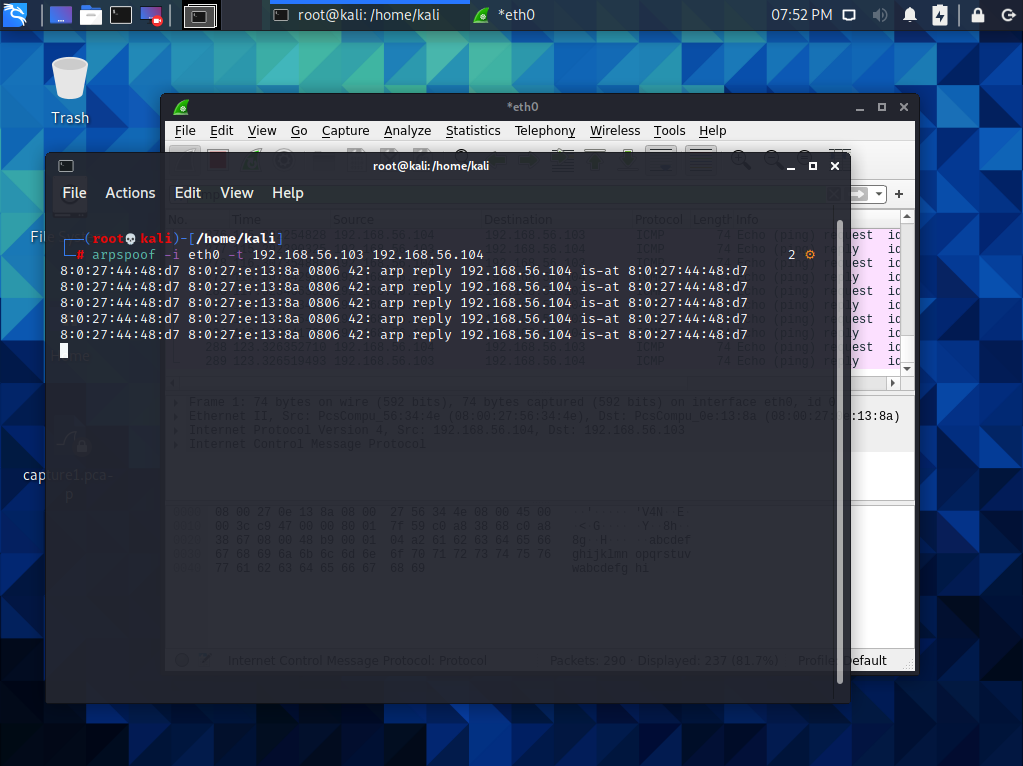
\includegraphics[width=\linewidth]{figures/arpspoof-initial.png}
    \caption{Running the first arpspoof command.}
    \label{fig:aprspoof-1}
\end{figure}

Wireshark now shows that the IP and MAC address are not the same as they were initially.
\begin{figure}[H]
    \centering
    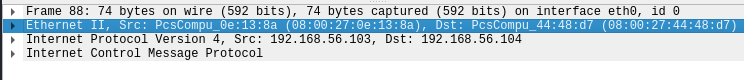
\includegraphics[width=\linewidth]{figures/wireshark-arp-1.png}
    \caption{Packet redirected to Kali machine}
    \label{fig:wireshark-redirect}
\end{figure}

Now we reverse the command to target the Windows-10 Clone machine.
This redirecting process means that the reply is lost, making the pings fail to deliver.
\begin{figure}[H]
    \centering
    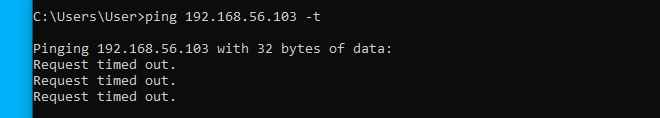
\includegraphics[width=\linewidth]{figures/ping-broken.png}
    \caption{Ping request timing out.}
    \label{fig:ping-fail}
\end{figure}

To fix this issue we enable port forwarding on Kali with \verb|echo 1 > /proc/sys/net/ipv4/ip_forward|.
Now the pings should be working.
\begin{figure}[H]
    \centering
    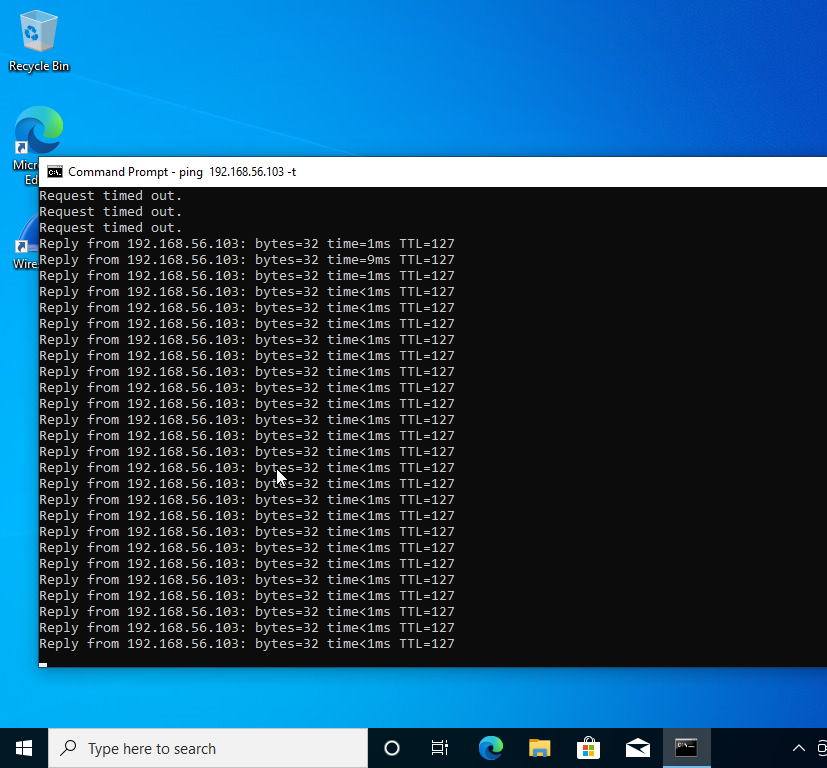
\includegraphics[width=\linewidth]{figures/ping-working-again.png}
    \caption{Pings have resumed.}
    \label{fig:ping-better}
\end{figure}

Now in Wireshark we see two requests and two replies:
\begin{figure}[H]
    \centering
    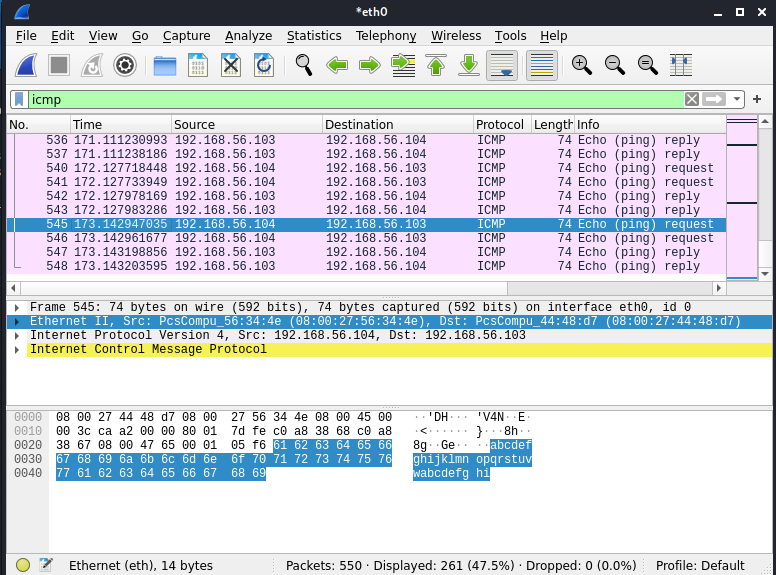
\includegraphics[width=\linewidth]{figures/request1.png}
    \caption{Request from Windows-10 to Kali.}
    \label{fig:request1}
\end{figure}
\begin{figure}[H]
    \centering
    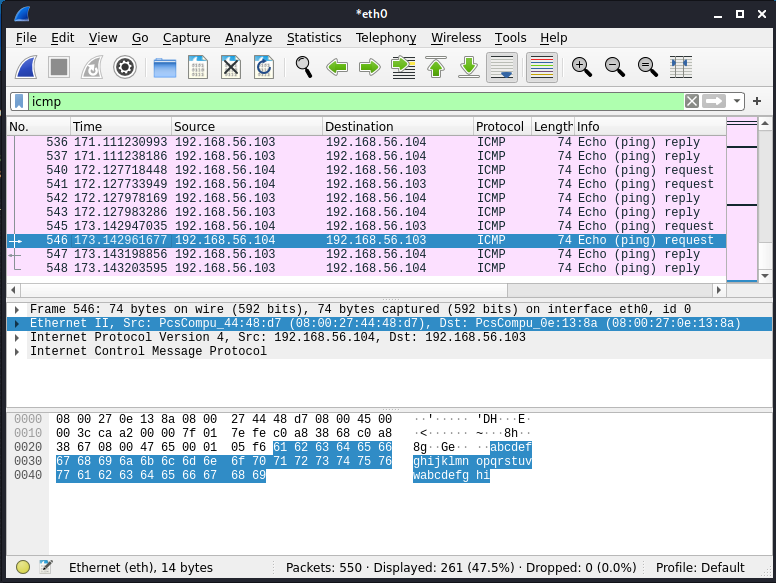
\includegraphics[width=\linewidth]{figures/request2.png}
    \caption{Request from Kali to Windows-10 Clone.}
    \label{fig:request2}
\end{figure}
\begin{figure}[H]
    \centering
    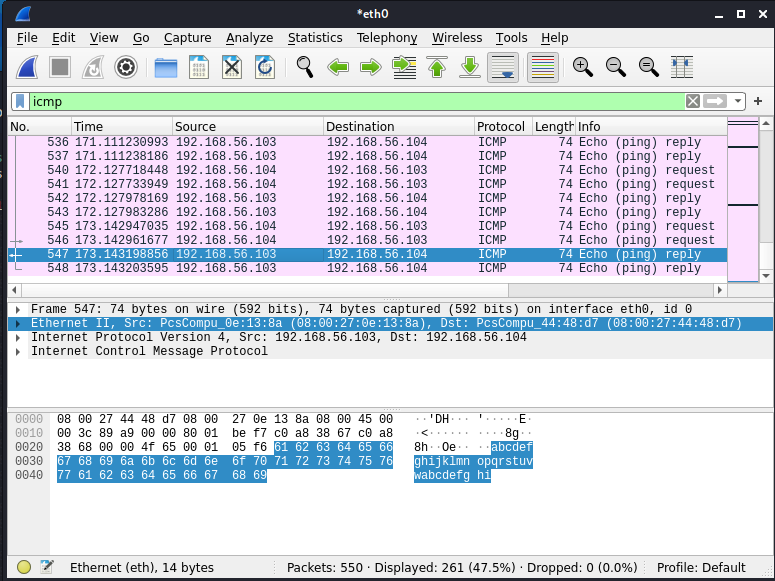
\includegraphics[width=\linewidth]{figures/reply1.png}
    \caption{Reply from Windows 10 Clone to Kali.}
    \label{fig:reply1}
\end{figure}
\begin{figure}[H]
    \centering
    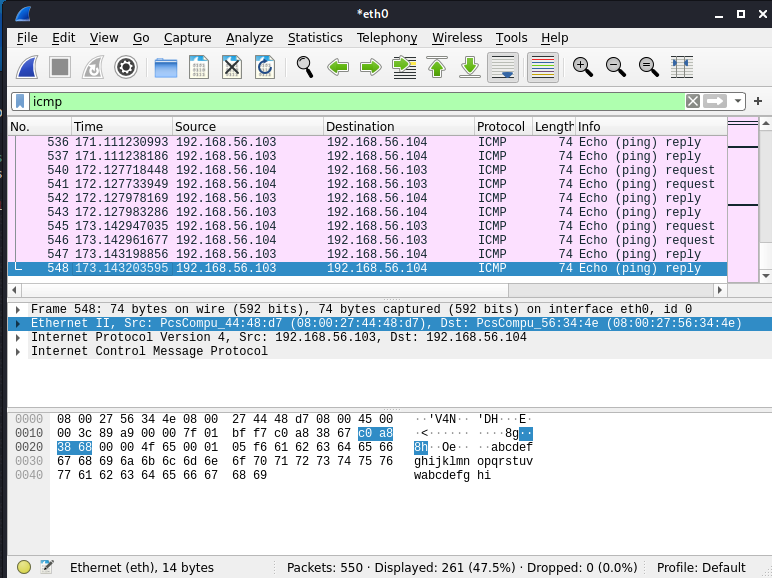
\includegraphics[width=\linewidth]{figures/reply2.png}
    \caption{Reply from Kali to Windows-10.}
    \label{fig:reply2}
\end{figure}

This lab demonstrates how an attacker can insert themselves in between network traffic to be a Man-in-the-Middle using ARP spoofing.
By infecting both the host and target machines, they are unable to differentiate a packet sent from them or from the attacker.
This allows the attacker to receive the packets sent from the host to the target and alter them en-route.
The same goes for communication between the target and the host.
The last 4 figures show that if someone is watching the network they could easily see that there are two sets of traffic and stop the attack.
However without the careful monitoring of the network, this attack would have gone unnoticed.